% cpu/overview.tex

\section{Overview}
\label{sec:cpu:Overview}

컴퓨터 시스템 스펙 문서를 생각없이 읽으면 CPU 성능이란
Figure~\ref{fig:cpu:CPU Performance at its Best} 에 그려진 것과 같은, 제일 빠른
사람이 항상 경주에서 이기는, 깨끗한 운동장에서의 도보 경주와 같다고 생각하기
쉽습니다.
\iffalse

Careless reading of computer-system specification sheets might lead one
to believe that CPU performance is a footrace on a clear track, as
illustrated in Figure~\ref{fig:cpu:CPU Performance at its Best},
where the race always goes to the swiftest.
\fi

\begin{figure}[htb]
\centering
\resizebox{3in}{!}{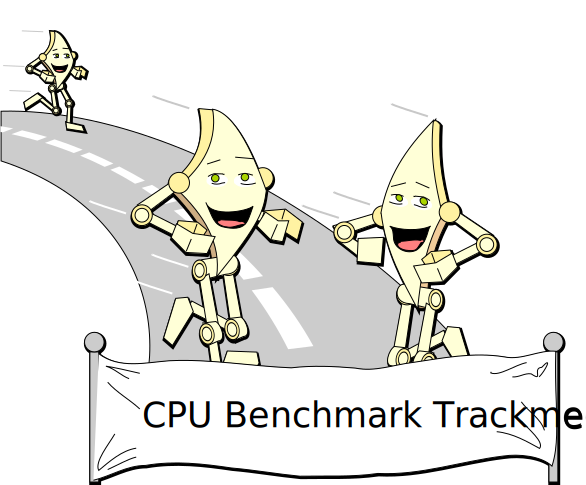
\includegraphics{cartoons/r-2014-CPU-track-meet}}
\caption{CPU Performance at its Best}
\ContributedBy{Figure}{fig:cpu:CPU Performance at its Best}{Melissa Broussard}
\end{figure}

Figure~\ref{fig:cpu:CPU Performance at its Best} 에 보여진 이상적 상황으로
접근하는 CPU 바운드 벤치마크들도 몇개 있긴 합니다만, 일반적인 프로그램은 경주용
운동장보다는 장애물 코스에 더 가깝습니다.
무어의 법칙에 의해 CPU 의 내부 구조가 지난 수십년간 엄청나게 변해왔기 때문이죠.
이런 변경들을 다음 섹션들에서 설명합니다.
\iffalse

Although there are a few CPU-bound benchmarks that approach the ideal
shown in Figure~\ref{fig:cpu:CPU Performance at its Best},
the typical program more closely resembles an obstacle course than
a race track.
This is because the internal architecture of CPUs has changed dramatically
over the past few decades, courtesy of Moore's Law.
These changes are described in the following sections.
\fi

\subsection{Pipelined CPUs}
\label{sec:cpu:Pipelined CPUs}

\begin{figure}[tb]
\centering
\resizebox{3in}{!}{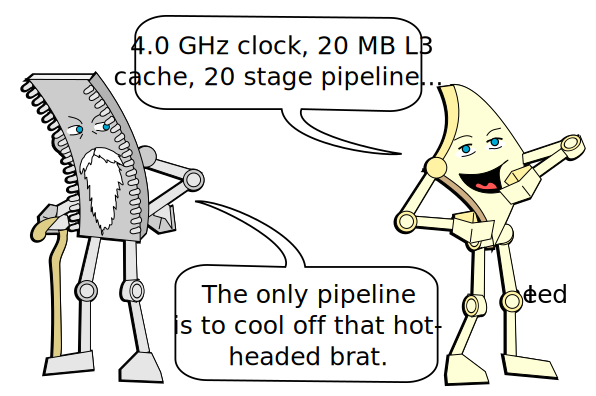
\includegraphics{cartoons/r-2014-Old-man-and-Brat}}
\caption{CPUs Old and New}
\ContributedBy{Figure}{fig:cpu:CPUs Old and New}{Melissa Broussard}
\end{figure}

1980년대 초, 인스트럭션을 가져오고, 디코드하고, 실행하는 대부분의 마이크로
프로세서는 일반적으로 다음 인스트럭션을 가져오기 전에 인스트럭션 하나를 실행
완료하는데 \emph{최소} 3 클락 사이클을 소모했습니다.
대조적으로, 1990년대 후반에서 2000년대 초반의 CPU 는 CPU 로의 인스트럭션 전달
흐름을 내부적으로 조절하는데 깊은 ``파이프라인'' 을 사용해 많은 인스트럭션들을
동시에 수행할 수 있습니다.
이러한 근래의 하드웨어의 기능들은 Figure~\ref{fig:cpu:CPUs Old and New} 에
보여진 것처럼 성능을 대폭 향상시킬 수 있습니다.

\iffalse
In the early 1980s, the typical microprocessor fetched an instruction,
decoded it, and executed it, typically taking \emph{at least} three
clock cycles to complete one instruction before proceeding to the next.
In contrast, the CPU of the late 1990s and early 2000s will be executing
many instructions simultaneously, using a deep ``pipeline'' to control
the flow of instructions internally to the CPU.
These modern hardware features can greatly improve performance, as
illustrated by Figure~\ref{fig:cpu:CPUs Old and New}.
\fi

긴 파이프라인을 가지고 CPU 의 최대 성능을 얻기 위해서는 프로그램의 컨트롤
플로우 (코드 실행 흐름)를 매우 정밀하게 예측할 수 있어야 합니다.
큰 행렬이나 벡터 계산과 같이 기본적으로 꽉 짜여진 루프로 구성된 프로그램에서는
적당한 컨트롤 플로우를 얻을 수 있습니다.
그런 경우 CPU 는 루프 마지막의, 루프 마지막의, 루프 처음으로 돌아갈지 루프를
빠져나갈지에 대한 분기  조건이 거의 항상 참일 거라는 것을 올바르게 예측해서
파이프라인이 꽉차 있게 해 CPU가 최대 속도로 돌아갈 수 있게 할겁니다.

\iffalse
Achieving full performance with a CPU having a long pipeline requires
highly predictable control flow through the program.
Suitable control flow can be provided by a program that executes primarily
in tight loops, for example, arithmetic on large matrices or vectors.
The CPU can then correctly predict that the branch at the end of the loop
will be taken in almost all cases,
allowing the pipeline to be kept full and the CPU to execute at full speed.
\fi

\begin{figure}[tb]
\centering
\resizebox{3in}{!}{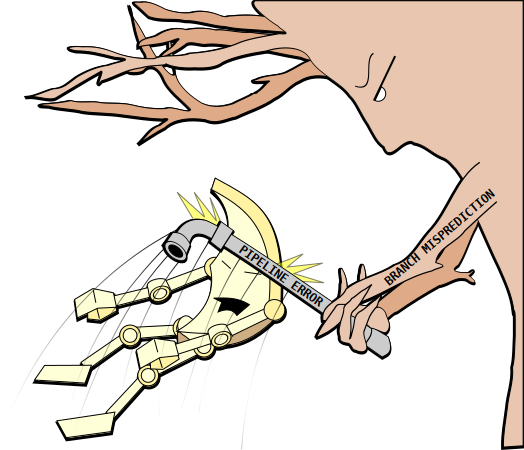
\includegraphics{cartoons/r-2014-branch-error}}
\caption{CPU Meets a Pipeline Flush}
\ContributedBy{Figure}{fig:cpu:CPU Meets a Pipeline Flush}{Melissa Broussard}
\end{figure}

하지만, 분기 예측이 항상 그렇게 쉬운건 아닙니다.
예를 들어, 작은 무작위적 횟수만큼 도는 많은 루프로 구성된 프로그램을
생각해보세요.
또다른 예로, 수많은 다른 진짜 객체를 레퍼런스 할 수 있는 가상 객체들이 있는데,
각 진짜 객체들은 자주 호출되는 멤버 함수들을 모두 다르게 구현한 객체지향
프로그램을 생각해보세요.
이런 경우, CPU 가 다음 분기가 실행 흐름을 어디로 이끌지를 예측하는것 조차도
불가능합니다.
그렇게 되면 CPU 는 그 브랜치가 어디로 실행 흐름을 이끌지가 확실해질 때까지
기다리며 멈춰있거나, 추측이라도 해야 합니다.
예측 가능한 컨트롤 플로우를 갖는 프로그램에서는 추측하는 방법이 매우 잘
동작하지만, (바이너리 서치와 같은) 예측 불가능한 분기분들에 대해서는 추측이
대부분 틀릴 겁니다.
추측이 잘못된 경우 CPU 는 그 분기문을 따르는, 투기적으로 그간 수행된
인스트럭션들을 모두 폐기시켜야 하기 때문에 파이프라인 플러시를 일으키기 때문에
잘못된 예측은 매우 비싼 비용을 지불합니다.
만약 파이프라인 플러시가 너무 자주 일어난다면, Figure~\ref{fig:cpu:CPU Meets a
Pipeline Flush} 에서 그려진 것처럼 엄청난 성능 하락을 겪을 수 있습니다.

\iffalse
However, branch prediction is not always so easy.
For example, consider a program with many loops, each of which iterates
a small but random number of times.
For another example, consider
an object-oriented program with many virtual objects that
can reference many different real objects, all with different implementations
for frequently invoked member functions.
In these cases, it is difficult or even
impossible for the CPU to predict where the next branch might lead.
Then either the CPU must stall waiting for execution to proceed far
enough to be certain where that branch leads, or it must guess.
Although guessing works extremely well for programs with predictable
control flow, for unpredictable branches (such as those in binary search)
the guesses will frequently be wrong.
A wrong guess can be expensive because the CPU must discard any
speculatively executed instructions following the corresponding
branch, resulting in a pipeline flush.
If pipeline flushes appear too frequently, they drastically reduce
overall performance, as fancifully depicted in
Figure~\ref{fig:cpu:CPU Meets a Pipeline Flush}.
\fi

불행히도, 파이프라인 플러시는 근래의 CPU 들이 달려야 하는 장애물 코스의 유일한
위험이 아닙니다.
다음 섹션에서는 메모리 참조에 존재하는 위험들을 다룹니다.

\iffalse
Unfortunately, pipeline flushes are not the only hazards in the obstacle
course that modern CPUs must run.
The next section covers the hazards of referencing memory.
\fi

\subsection{Memory References}
\label{sec:cpu:Memory References}

1980년대에는, 대부분의 경우 마이크로프로세서가 메모리에서 값을 하나 얻어오는데
걸리는 시간이 인스트럭션 하나를 수행하는데 걸리는 시간보다 적었습니다.
2006년에 와서는, 마이크로프로세서는 메모리에 접근 한번 하는데 걸리는 시간 동안
수백, 심한 경우 수천개의 인스트럭션을 수행할 수 있습니다.
이 간극은 Moore 의 법칙이 CPU 성능 향상을 메모리 반응속도의 감소 정도에 비해
너무 크게 이끌었기 때문입니다; 메모리의 발전은 반응속도 감소보다 용량 증가에
치중되었던 것도 한 이유죠.
예를 들어, 1970년대의 평범한 미니컴퓨터는 4KB (네, 메가바이트가 아니라
킬로바이트요. 기가바이트는 입밖에 꺼내지도 마요) 메인 메모리를 가졌고, 그
메모리는 한 사이클만에 접근 가능했습니다.\footnote{
	물론 그 한개의 사이클은 1.6 \emph{마이크로 세컨드} 이상이었음을
	언급하는게 공정하겠죠.}
2008년에도 CPU 설계자들은 여전히 단일 사이클만에 접근 가능한 4KB 메모리를 만들
수 있습니다; 심지어 수 GHz 주파수의 시스템에서도요.
그리고 실제로 그런 메모리를 만듭니다만, 그들은 이제 그걸 ``레벨 0 캐시'' 라
부르고, 그것들은 보통은 4KB 보다는 아주 약간은 크기도 합니다.

\iffalse
In the 1980s, it often took less time for a microprocessor to load a value
from memory than it did to execute an instruction.
In 2006, a microprocessor might be capable of executing hundreds or even
thousands of instructions in the time required to access memory.
This disparity is due to the fact that Moore's Law has increased CPU
performance at a much greater rate than it has decreased memory latency,
in part due to the rate at which memory sizes have grown.
For example, a typical 1970s minicomputer might have 4\,KB (yes, kilobytes,
not megabytes, let alone gigabytes) of main memory, with
single-cycle access.\footnote{
	It is only fair to add that each of these single cycles
	lasted no less than 1.6 \emph{microseconds}.}
In 2008, CPU designers still can construct a 4\,KB memory with single-cycle
access, even on systems with multi-GHz clock frequencies.
And in fact they frequently do construct such memories, but they now
call them ``level-0 caches'', and they can be quite a bit bigger than 4\,KB.
\fi

\begin{figure}[htb]
\centering
\resizebox{3in}{!}{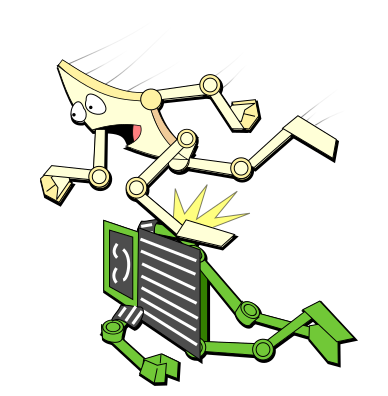
\includegraphics{cartoons/r-2014-memory-reference}}
\caption{CPU Meets a Memory Reference}
\ContributedBy{Figure}{fig:cpu:CPU Meets a Memory Reference}{Melissa Broussard}
\end{figure}

근래의 마이크로프로세서에 장착되는 큰 캐시들은 메모리 접근 시간과 맞서 싸우는데
꽤 도움을 줄 수 있습니다만, 이런 캐시들이 그 시간들을 제대로 숨기기 위해서는
고도로 예측 가능한 데이터 접근 패턴이 필요합니다.
불행히도, 링크드 리스트를 순회하는 것과 같은 많은 일들이 예측 불가능한 메모리
접근 패턴을 갖습니다. 무엇보다, 만약 패턴이 예측 가능하다면, 소프트웨어는
포인터 타입이란 것 자체를 만들지도 않았겠죠, 그렇죠?
따라서, Figure~\ref{fig:cpu:CPU Meets a Memory Reference} 에서 보여지듯, 메모리
참조는 종종 근래의 CPU 들에게 거대한 장애물입니다.

지금까지는 주어진 CPU가 싱글 쓰레드 코드를 돌릴 때 만날 수 있는 문제들만
이야기했습니다.
멀티쓰레드 수행은 다음 섹션에서 설명할텐데, 추가적인 문제들을 CPU 에게
내놓습니다.

\iffalse
Although the large caches found on modern microprocessors can do quite
a bit to help combat memory-access latencies,
these caches require highly predictable data-access patterns to
successfully hide those latencies.
Unfortunately, common operations such as traversing a linked list
have extremely unpredictable memory-access patterns---after all,
if the pattern was predictable, us software types would not bother
with the pointers, right?
Therefore, as shown in
Figure~\ref{fig:cpu:CPU Meets a Memory Reference},
memory references often pose severe obstacles to modern CPUs.

Thus far, we have only been considering obstacles that can arise during
a given CPU's execution of single-threaded code.
Multi-threading presents additional obstacles to the CPU, as
described in the following sections.
\fi

\subsection{Atomic Operations}
\label{sec:cpu:Atomic Operations}

그런 장애 중 하나는 어토믹 오퍼레이션들입니다.
여기서의 문제는 모든 어토믹 오퍼레이션은 CPU 파이프라인의 한 순간에는 조각으로
나뉘어 수행되는 어셈블리 오퍼레이션들과 한번씩은 충돌한다는 것입니다.
하드웨어 설계자는 근래의 CPU 들은 그런 오퍼레이션들이 실은 여러 조각으로
나뉘어져 여러 순간동안 수행되더라도 원자적으로 수행되는 것처럼 \emph{보이게}
하기 위해 여러개의 굉장히 현명한 트릭들을 사용한다고 이야기합니다. 그런 트릭 중
흔한 한가지는 어토믹하게 수행되어야 하는 데이터를 담고 있는 캐시라인들을 모두
파악해두고, 이 캐시라인들은 해당 어토믹 오퍼레이션을 수행하는 CPU 에 소유되어
있음을 분명하게 하고, 그러고나서야만 해당 캐시라인들이 해당 CPU 에 의해 여전히
소유되어 있음을 분명히 한 채로 어토믹 오퍼레이션을 수행하는 것입니다.
모든 데이터가 해당 CPU 만 접근할 수 있는 상태이기에, 다른 CPU 들은 실은
조각으로 나뉘어 수행되는 CPU 파이프라인의 현실에도 불구하고 해당 어토믹
오퍼레이션에 간섭을 끼칠 수 없습니다.
말할 필요도 없겠지만, 이런 종류의 트릭은 그 셋업이 수행되도록 주어진 어토믹
오퍼레이션이 완전히 끝날 때까지 파이프라인이 지연되거나 심지어 플러시될 수도
있습니다.

\iffalse
One such obstacle is atomic operations.
The problem here is that the whole idea of an atomic operation conflicts with
the piece-at-a-time assembly-line operation of a CPU pipeline.
To hardware designers' credit, modern CPUs use a number of extremely clever
tricks to make such operations \emph{look} atomic even though they
are in fact being executed piece-at-a-time,
with one common trick being to identify all the cachelines containing the
data to be atomically operated on,
ensure that these cachelines are owned by the CPU executing the
atomic operation, and only then proceed with the atomic operation
while ensuring that these cachelines remained owned by this CPU.
Because all the data is private to this CPU, other CPUs are unable to
interfere with the atomic operation despite the piece-at-a-time nature
of the CPU's pipeline.
Needless to say, this sort of trick can require that
the pipeline must be delayed or even flushed in order to
perform the setup operations that
permit a given atomic operation to complete correctly.
\fi

\begin{figure}[htb]
\centering
\resizebox{3in}{!}{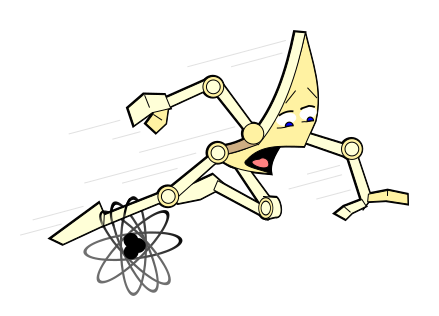
\includegraphics{cartoons/r-2014-Atomic-reference}}
\caption{CPU Meets an Atomic Operation}
\ContributedBy{Figure}{fig:cpu:CPU Meets an Atomic Operation}{Melissa Broussard}
\end{figure}

반대로, 어토믹 오퍼레이션이 아닌 오퍼레이션을 수행할 때에는 CPU 는 값을
캐시라인에 올라오는대로 가져올 수 있고, 수행 결과를 캐시라인 소유권을 가지기
위해 기다릴 필요 없이 곧바로 버퍼에 써넣을 수 있습니다.
다행히도, CPU 설계자들은 어토믹 오퍼레이션에 신경을 많이 쏟았고, 덕분에 2014년
초에 이르러서는 그 오버헤드를 상당히 감소시켰습니다.
하지만 그래도, 그 성능에 끼치는 효과는 Figure~\ref{fig:cpu:CPU Meets an Atomic
Operation} 에 보이는 대로입니다.

불행히도, 어토믹 오퍼레이션들은 보통 데이터의 한개 요소에만 적용 가능합니다.
많은 병렬 알고리즘들이 복수개의 데이터 요소들에의 업데이트 간에도 순서가
이루어지길 필요로 하기 때문에, 대부분의 CPU 들은 메모리 배리어들을 제공합니다.
이런 메모리 배리어들 역시 성능에의 문제로 존재합니다. 다음 섹션에서 이를 이야기
합니다.

\iffalse
In contrast, when executing a non-atomic operation, the CPU can load
values from cachelines as they appear and place the results in the
store buffer, without the need to wait for cacheline ownership.
Fortunately, CPU designers have focused heavily on atomic operations,
so that as of early 2014 they have greatly reduced their overhead.
Even so, the resulting effect on performance is all too often as depicted in
Figure~\ref{fig:cpu:CPU Meets an Atomic Operation}.

Unfortunately, atomic operations usually apply only to single elements
of data.
Because many parallel algorithms require that ordering constraints
be maintained between updates of multiple data elements, most CPUs
provide memory barriers.
These memory barriers also serve as performance-sapping obstacles,
as described in the next section.
\fi

\QuickQuiz{}
	어떤 기계가 복수 데이터 요소에 대한 어토믹 오퍼레이션을 허용하겠어요?

	\iffalse
	What types of machines would allow atomic operations on
	multiple data elements?
	\fi
\QuickQuizAnswer{
	이 질문에 대한 한가지 답은 종종 복수개의 데이터 요소를 어토믹하게
	다뤄질 수 있는, 단일 머신 워드 안에 모아넣을 수 있다는 겁니다.

	좀 더 트렌디한 답은 트랜잭셔널 메모리~\cite{DBLomet1977SIGSOFT} 를
	지원하는 기계가 되겠습니다.
	2014년 초에 이르러서는 일부 주요 시스템들이 제한되긴 했지만 하드웨어
	트랜잭셔널 메모리 구현을 제공합니다. 더 자세한 내용은
	Section~\ref{sec:future:Hardware Transactional Memory} 에서 다루고
	있습니다.
	소프트웨어 트랜잭셔널
	메모리~\cite{McKenney2007PLOSTM,DonaldEPorter2007TRANSACT,
	ChistopherJRossbach2007a,CalinCascaval2008tmtoy,
	AleksandarDragovejic2011STMnotToy,AlexanderMatveev2012PessimisticTM}
	에 대해서는 아직 적합하지 않다는 평가입니다.
	소프트웨어 트랜잭셔널 메모리에 대한 더 많은 내용은
	Section~\ref{sec:future:Transactional Memory} 에서 볼 수 있을 겁니다.

	\iffalse
	One answer to this question is that it is often possible to
	pack multiple elements of data into a single machine word,
	which can then be manipulated atomically.

	A more trendy answer would be machines supporting transactional
	memory~\cite{DBLomet1977SIGSOFT}.
	As of early 2014, several mainstream systems provide limited
	hardware transactional memory implementations, which is covered
	in more detail in
	Section~\ref{sec:future:Hardware Transactional Memory}.
	The jury is still out on the applicability of software transactional
	memory~\cite{McKenney2007PLOSTM,DonaldEPorter2007TRANSACT,
	ChistopherJRossbach2007a,CalinCascaval2008tmtoy,
	AleksandarDragovejic2011STMnotToy,AlexanderMatveev2012PessimisticTM}.
	Additional information on software transactional memory may be
	found in
	Section~\ref{sec:future:Transactional Memory}.
	\fi
} \QuickQuizEnd

\subsection{Memory Barriers}
\label{sec:cpu:Memory Barriers}

메모리 배리어에 대해서는
Chapter~\ref{chp:Advanced Synchronization: Memory Ordering} 와
Appendix~\ref{chp:app:whymb:Why Memory Barriers?} 에서 좀 더 깊게 다룰 겁니다.
그 전에, 여기서는 다음의 간단한 락을 사용한 크리티컬 섹션을 생각해 봅시다:

\iffalse
Memory barriers will be considered in more detail in
Chapter~\ref{chp:Advanced Synchronization: Memory Ordering} and
Appendix~\ref{chp:app:whymb:Why Memory Barriers?}.
In the meantime, consider the following simple lock-based critical
section:
\fi

\vspace{5pt}
\begin{minipage}[t]{\columnwidth}
\small
\begin{verbatim}
  1 spin_lock(&mylock);
  2 a = a + 1;
  3 spin_unlock(&mylock);
\end{verbatim}
\end{minipage}
\vspace{5pt}

\begin{figure}[tb]
\centering
\resizebox{3in}{!}{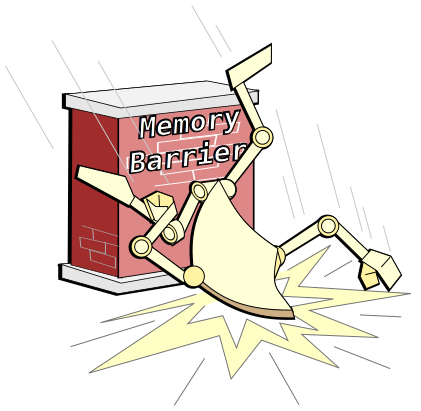
\includegraphics{cartoons/r-2014-Memory-barrier}}
\caption{CPU Meets a Memory Barrier}
\ContributedBy{Figure}{fig:cpu:CPU Meets a Memory Barrier}{Melissa Broussard}
\end{figure}

만약 CPU 에 코드가 보여지는 순서대로 수행되어야 한다는 제약이 존재하지
않는다면, 변수 ``a'' 는 ``mylock'' 의 보호 없이 값이 증가할 것이고, 이렇게 되면
락을 잡는 목표가 이뤄지지 않은 셈입니다.
그런 문제되는 순서 재배치를 막기 위해, 락킹에 사용되는 기본 기능들은 명시적이든
묵시적이든 메모리 배리어를 사용합니다.
이런 메모리 배리어의 목적은 CPU 가 성능을 향상시키기 위해 할 수 있는 코드의
순서 재배치를 막기 위한 것이기 때문에, 메모리 배리어는 거의 항상
Figure~\ref{fig:cpu:CPU Meets a Memory Barrier} 에서 보여지듯 성능을
떨어뜨립니다.

어토믹 오퍼레이션과 같이, CPU 설계자들은 메모리 배리어 오버헤드를 줄이려 열심히
노력해왔고, 꽤 많은 진전을 이뤘습니다.

\iffalse
If the CPU were not constrained to execute these statements in the
order shown, the effect would be that the variable ``a'' would be
incremented without the protection of ``mylock'', which would certainly
defeat the purpose of acquiring it.
To prevent such destructive reordering, locking primitives contain
either explicit or implicit memory barriers.
Because the whole purpose of these memory barriers is to prevent reorderings
that the CPU would otherwise undertake in order to increase performance,
memory barriers almost always reduce performance, as depicted in
Figure~\ref{fig:cpu:CPU Meets a Memory Barrier}.

As with atomic operations, CPU designers have been working hard to
reduce memory-barrier overhead, and have made substantial progress.
\fi

\subsection{Cache Misses}
\label{sec:cpu:Cache Misses}

\begin{figure}[tb]
\centering
\resizebox{3in}{!}{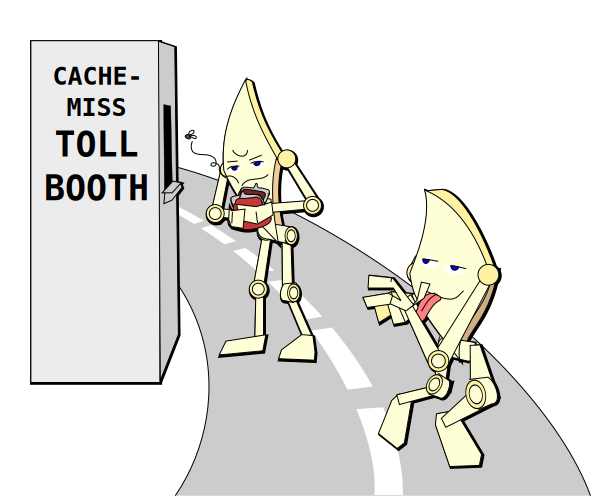
\includegraphics{cartoons/r-2014-CPU-track-meet-cache-miss-toll-booth}}
\caption{CPU Meets a Cache Miss}
\ContributedBy{Figure}{fig:cpu:CPU Meets a Cache Miss}{Melissa Broussard}
\end{figure}

또하나의 멀티 쓰레딩에서의 CPU 성능에의 장애물은 ``캐시 미스'' 입니다.
앞서 말했듯, 근래의 CPU 들은 높은 메모리 반응속도로 발생할 수 있는 성능 하락을
줄이기 위해 큰 캐시를 장착하고 있습니다.
하지만, 이런 캐시들은 실은 CPU 간에 자주 공유되는 변수들에 대해서는 생산적이지
못합니다.
하나의 CPU 가 한 변수를 수정하려 할 때, 다른 CPU 가 그 값을 최근에 바꾼 경우가
있을 가능성이 크기 때문이죠.
이런 경우, 해당 변수는 지금 수정하려는 CPU 의 캐시가 아니라 최근에 값을 수정한
CPU 의 캐시에 있을 것이고, 이로 인해 비싼 캐시 미스(더 자세한 내용을 위해선
Section~\ref{sec:app:whymb:Cache Structure} 를 보세요) 를 일으킬 것입니다.
이런 캐시 미스들은 Figure~\ref{fig:cpu:CPU Meets a Cache Miss} 에서 보여진
것처럼 CPU 성능의 주요 장애가 됩니다.

\iffalse
An additional multi-threading obstacle to CPU performance is
the ``cache miss''.
As noted earlier, modern CPUs sport large caches in order to reduce the
performance penalty that would otherwise be incurred due to high memory
latencies.
However, these caches are actually counter-productive for variables that
are frequently shared among CPUs.
This is because when a given CPU wishes to modify the variable, it is
most likely the case that some other CPU has modified it recently.
In this case, the variable will be in that other CPU's cache, but not
in this CPU's cache, which will therefore incur an expensive cache miss
(see Section~\ref{sec:app:whymb:Cache Structure} for more detail).
Such cache misses form a major obstacle to CPU performance, as shown
in Figure~\ref{fig:cpu:CPU Meets a Cache Miss}.
\fi

\QuickQuiz{}
	그래서, CPU 설계자들은 캐시 미스 오버헤드 역시 많이 개선 했나요?
	\iffalse
	So have CPU designers also greatly reduced the overhead of
	cache misses?
	\fi
\QuickQuizAnswer{
	안타깝지만, 그렇게 많은 개선은 하지 못했습니다.
	약간 오버헤드를 줄인 CPU 들도 있었습니다만, 빛의 속도의 한계와 물질의
	원자성의 자연 법칙이 큰 시스템에서 캐시 미스 오버헤드를 줄일 수 있는
	방법을 제한하고 있습니다.
	Section~\ref{sec:cpu:Hardware Free Lunch?} 에서 가능할 법한 미래의 개선
	방법들을 논의해 봅니다.

	\iffalse
	Unfortunately, not so much.
	There has been some reduction given constant numbers of CPUs,
	but the finite speed of light and the atomic nature of
	matter limits their ability to reduce cache-miss overhead
	for larger systems.
	Section~\ref{sec:cpu:Hardware Free Lunch?}
	discusses some possible avenues for possible future progress.
	\fi
} \QuickQuizEnd

\subsection{I/O Operations}
\label{sec:cpu:I/O Operations}

\begin{figure}[tb]
\centering
\resizebox{3in}{!}{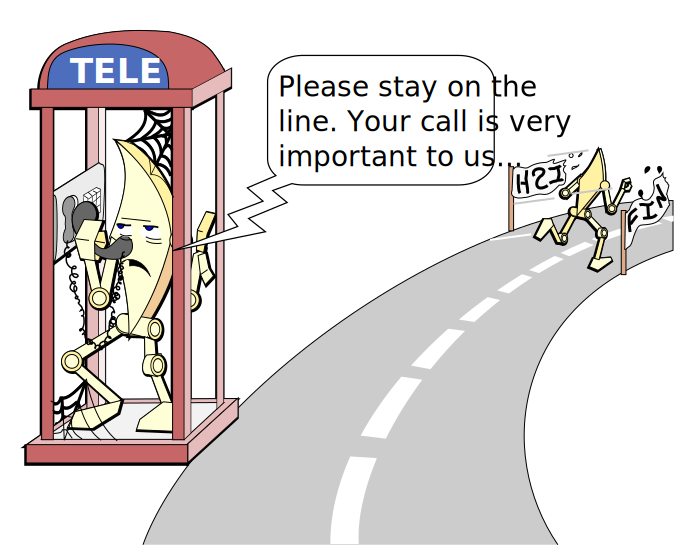
\includegraphics{cartoons/r-2014-CPU-track-meet-phone-booth}}
\caption{CPU Waits for I/O Completion}
\ContributedBy{Figure}{fig:cpu:CPU Waits for I/O Completion}{Melissa Broussard}
\end{figure}

캐시 미스는 곧 CPU 와 CPU 사이의 I/O 오퍼레이션으로 볼 수 있고, 이것은 가능한
I/O 오퍼레이션 중 가장 비용이 낮은 것들 중 하나입니다.
네트워킹이나 대용량 저장장치, 또는 사람을 포함하는 I/O 오퍼레이션들은
Figure~\ref{fig:cpu:CPU Waits for I/O Completion} 에서 보여지듯, 앞의
섹션들에서 이야기 되었던 내부적 장애들보다 훨씬 커다란 장애를 야기합니다.

\iffalse
A cache miss can be thought of as a CPU-to-CPU I/O operation, and as
such is one of the cheapest I/O operations available.
I/O operations involving networking, mass storage, or (worse yet) human
beings pose much greater obstacles than the internal obstacles called
out in the prior sections,
as illustrated by
Figure~\ref{fig:cpu:CPU Waits for I/O Completion}.
\fi

이건 공유 메모리 병렬성과 분산시스템 병렬성 사이의 차이 중 하나입니다:
공유메모리 병렬 프로그램은 일반적으로 캐시 미스보다 더한 장애는 겪지
않습니다만, 분산 병렬 프로그램은 보통 더 큰 네트워크 커뮤니케이션 시간을
겪습니다.
두 경우 모두, 문제의 응답시간들은 커뮤니케이션의 비용으로 생각될 수 있습니다.
순차 프로그램에서는 존재하지 않는 비용이죠.
따라서, 실제 수행되는 일과 커뮤니케이션 오버헤드 간의 비율이 핵심 설계 결정
요소입니다.
병렬 하드웨어 설계의 주요 목표는 이 비율을 적절한 성능과 확장성 목표를 달성
가능한 수준으로 낮추는 것입니다.
이에 따라서, Chapter~\ref{cha:Partitioning and Synchronization Design} 에서
볼테지만, 병렬 소프트웨어 설계의 중요한 목표는 커뮤니케이션 캐시 미스와 같은
비싼 동작들의 빈번도를 낮추는 것입니다.

물론, 주어진 동작이 장애라는 이야기는 그 이야기이고, 그 동작이 \emph{심각한}
장애라는 건 또 따로 보여줘야하지요.
이 차이를 다음의 섹션에서 이야기 합니다.

\iffalse
This is one of the differences between shared-memory and distributed-system
parallelism: shared-memory parallel programs must normally deal with no
obstacle worse than a cache miss, while a distributed parallel program
will typically incur the larger network communication latencies.
In both cases, the relevant latencies can be thought of as a cost of
communication---a cost that would be absent in a sequential program.
Therefore, the ratio between the overhead of the communication to
that of the actual work being performed is a key design parameter.
A major goal of parallel hardware design is to reduce this ratio as
needed to achieve the relevant performance and scalability goals.
In turn, as will be seen in
Chapter~\ref{cha:Partitioning and Synchronization Design},
a major goal of parallel software design is to reduce the
frequency of expensive operations like communications cache misses.

Of course, it is one thing to say that a given operation is an obstacle,
and quite another to show that the operation is a \emph{significant}
obstacle.
This distinction is discussed in the following sections.
\fi
